\documentclass[a4paper, 11pt, tikz]{article}

% Toggle switch for moving tables and figures at the back + placing markers in the body text
\usepackage[fighead, notabhead, nolists]{endfloat}
\renewcommand{\figuresection}{Figures and Tables}

\newenvironment{ltable}
  {\begin{landscape}}
  {\end{landscape}}
\DeclareDelayedFloatFlavour{ltable}{table}

\usepackage{tikz}
\usepackage{tikz-qtree}

\usepackage{pdflscape}

\usepackage{subcaption}
\captionsetup[sub]{font=footnotesize, labelfont={bf,sf}} % 8pt for subcaptions

%% AMS mathematics packages - they contain many useful fonts and symbols.
\usepackage{amsmath, amsfonts, amssymb, amsthm, mathtools}
\usepackage{float}
% \floatplacement{figure}{H}
% \floatplacement{table}{H}

\usepackage{graphicx}

\usepackage{bbm}
\usepackage{physics}

\usepackage{setspace}
\usepackage{natbib}
\usepackage{tabularx}

\usepackage{tabularray}
\usepackage{codehigh}
\usepackage[normalem]{ulem}
\UseTblrLibrary{booktabs}
\UseTblrLibrary{siunitx}
\newcommand{\tinytableTabularrayUnderline}[1]{\underline{#1}}
\newcommand{\tinytableTabularrayStrikeout}[1]{\sout{#1}}
\NewTableCommand{\tinytableDefineColor}[3]{\definecolor{#1}{#2}{#3}}

\usepackage[usestackEOL]{stackengine}

\usepackage[paper=a4paper, left=2.54cm, right=2.54cm, top=2.54cm, bottom=2.54cm]{geometry}

\usepackage{url}
\sloppy
\def\UrlBreaks{\do\/\do-}
\usepackage[breaklinks]{hyperref}
\usepackage{breakurl}

% \usepackage{newtxtext} % Use Times Roman font
% \usepackage{newtxmath} % Use Times Roman font
\usepackage[T1]{fontenc}
\usepackage{newpxtext, newpxmath}

\newcommand{\E}{\mathbb{E}}

\begin{document}
\begin{titlepage}
\title{Jobless Unemployed Workers and Temporary Layoff Workers on Search and Not on Search for a New Job in the US Labour Market\thanks{I would like to express my gratitude to Prof Jesper Bagger for his continual supervision of this reserach. I am also grateful to my parents who have given me an invaluable opportunity to pursue my undergraduate studies away from home. All remaining errors are my own.}}
\author{Exam Number: B209498}
\date{13 April 2025 \vskip \baselineskip Word Count: 9953}
\maketitle
\begin{abstract}
\noindent The empirical literature has documented a significant proportion of temporary layoff workers in the US labour market and their systematic differences to other unemployed workers.
Temporary layoff workers are the unemployed with a specific return date to their last firm or at least an indication to be recalled within six months, unlike the other types of unemployment. Individual differences of those two types of unemployed workers are explored using longitudinally linked Current Population Survey data.
Furthermore, I focus on the heterogeneity within temporary layoff workers that some look for an alternative job while the others do not.
I find temporary layoff workers' decisions to search a new job are related to their job-finding rates and individual attributes, calling for a need to distinguish between them in analysing heterogeneous unemployment.
Furthermore, I estimate an extended model of the labour matching function that predicts the number of new hires from vacancy counts as well as from separate levels of unemployment in different types.
OLS estimates suggest a continuing decline in matching efficiency after the 2008 recession is partly due to a decreasing share of temporary layoff workers, but they may contain endogenous biases. \\
\vspace{0in}\\
\noindent\textbf{Keywords:} Temporary layoff, matching function, job-finding rate\\
\vspace{0in}\\
\noindent\textbf{JEL Codes:} J63, J64, E24\\

\bigskip
\end{abstract}
\setcounter{page}{0}
\thispagestyle{empty}
\end{titlepage}
\pagebreak \newpage

\pagenumbering{roman}
\tableofcontents
\listoffigures
\listoftables

\pagebreak \newpage

\pagenumbering{arabic}
\onehalfspacing

\section{Introduction}
In the labour market in the US and in other developed economies, there has been a considerable proportion of temporary layoff workers, who have a specific return date or are given an indication to be recalled by the last employer.
Those workers differ systematically from permanently laid-off workers, while their difference and its significance have often been overlooked in the labour economics literature.
This paper will focus on the difference between those two different types of unemployed workers in the US labour market and examine the impact of this heterogeneity on job-search consequences of the unemployed workers.

I use the Current Population Survey (CPS) data in the US, and hence, follow its definition for the distinction between temporary-layoff (TL) and jobless (JL) unemployment: the former indicates people who are on layoff with a specific return date to the last employer or with an indication given by the last employer of recall within the next six months; the latter for those without a specific return date nor an indication to be recalled.
One notable difference between TL and JL unemployment is that, while JL unemployed workers are assumed to be actively looking for new jobs, TL workers are not, resulting in some proportion of furloughed workers not actively looking for an alternative job.
Along with the distinction between TL and JL unemployment, this paper also focuses on the different characteristics of those who are searching and not searching among TL unemployed workers.

As an attempt to show the importance of differently treating furloughed workers (who are either searching or not) from the entire unemployed population, I revisit a matching function in the labour market, a commonly used function to simplify the matching process between workers and firms.
Compared to a canonical model of the matching function that determines the number of new hires from an aggregated level of unemployment and vacancy counts, I propose an extension that separately treats different types of unemployment in the input of the function.
Furthermore, while the literature suggests basic OLS estimates of a matching function may suffer from an endogeneity bias, I employ instrumental variable approach to examine if this issue can be resolved.

The rest of the paper is organised as follows.
First, the labour economics literature on temporary layoff and on estimating matching functions is explored.
Second, I describe the data utilised in the analysis and provide descriptive statistics on the TL unemployed workers to reassure the importance of distinctive treatment according to the types of unemployment.
Third, different models to estimate a matching function are presented with an emphasis on an endogenous bias that the most basic model estimation may suffer.
Then, estimation results are presented and compared with that of a couple of alternative models.
Finally, the paper discusses the results and concludes with suggesting possible areas to be addressed in future research.

\section{Literature}
\subsection{Temporary Layoff Unemployment}
Empirical literature documents there have consistently been a significant proportion of TL workers in the unemployment population and TL workers have had systematically different characteristics to the unemployed of the other types.
Furthermore, researchers have found that returning to the last employer after a period of unemployment is also common among JL unemployed workers who were initially not expected to be recalled.
In the US labour market, \cite{fujita2017recall} report that TL workers tend to have had a longer tenure length at the last employer, experience a shorter unemployment period by more than a month, and once they are recalled by the previous firm, they tend to stay longer and switch to another job much less often than JL workers.
They use the Survey of Income and Program Participation (SIPP) data from 1990 to 2013 for their analysis and point out that 40\% of the separated workers returned to their last employer.
Older literature documented similar figures, namely \cite{katz1990impact} using unemployment insurance (UI) recipients data in Missouri and Pennsylvania between 1979 and 1981.
They found 72\% of the UI recipients with an initial expectation to be recalled were actually recalled, and 13\% of those without an indication of recall indeed returned to the last employer.
Outside the US, \cite{nekoei2015recall} analysed Austrian administrative data from 2004 to 2013, documenting that 42\% of all separations were temporary layoffs, and 58\% of TL workers and 19\% of those initially permanently separated were recalled.
Their paper is followed up by \cite{nekoei2020seven} using the same data, finding that when TL share is higher at a firm or in an industry, both TL and JL separated workers could expect a higher rate of future recall.
Also, \cite{nekoei2020seven} suggest that TL is more common among workers in upper-middle part of the wage distribution as well as during recession, the latter of which agrees with the finding by \cite{fujita2017recall}.

Those empirical findings of temporary layoffs and firms' recalling behaviour have recently been actively incorporated in search and matching models to investigate in relation to business cycle fluctuations.
\cite{fujita2017recall}, who acknowledge the significance of layoff recalls by analysing the SIPP data, were the first to extend a stochastic Diamond-Mortensen-Pissarides (DMP) search model to incorporate a recall option for firms as follows.
First, firms in the model may suspend production due to an aggregate shock and subsequently lay off some of their employees.
Then, those furloughed workers will start looking for another job with a search cost, while firms that are to resume production can also spend costs in posting job vacancies to seek a match with new workers.
However, departure from the original DMP model is that the employer can also use a ``recall'' option, calling previous employees to return to them at no matching cost on both sides, given they have not made a new match with another employer yet.

While the \cite{fujita2017recall} model successfully captures the movement of workers across employment status in the US labour market, further modifications have been made to adjust contradictions against observations in the real economy and reflect findings in the empirical literature in more detail.
Notably, since \cite{fujita2017recall} simply added a recall option that can be exercised for all the previous workers on furlough, their model fails in differentiating TL unemployed workers from the JL unemployed, which should be explicit at the time of separation by firms giving a specific date to return or at least an indication to recall to their workers entering TL.
\cite{gertler2022temporary} incorporate this and let a firm decide whether the layoff will be temporary or permanent at the time of separation endogenously determined by overhead costs and value of matches built individually with their workers.
Similar approach is taken by \cite{gallant2020temporary} and \cite{komatsu2024temporary}.

Those estimated search and matching models with incorporating temporary layoffs are applied both in theoretical and empirical studies.
First, \cite{komatsu2024temporary} simulates the model to assess the impact of unemployment insurance (UI) on job search behaviour and firms' temporary layoff decisions.
The author constructs a model in which the unemployed workers lose eligibility for UI benefits at some probability each period, finding that generous UI benefits increase the share of TL and extend the spell of temporary layoff, while they decrease the job-finding rate among TL workers; those findings are compatible with the author's empirical evidence based on CPS data.
Second, several papers acknowledge that the shock of the Covid-19 pandemic to the labour market was peculiar in terms of temporary layoff as well, in that labour market observed temporary layoffs from the onset of the pandemic, while past recessions began with an increase in permanent layoffs \citep{gallant2020temporary}.
In addition, TL share indeed accounted for almost the entire job separation in the first few months of the recession, which may have accelerated unemployment recovery to a faster-than-history level \citep{gallant2020temporary, hall2022unemployed}.
Particularly, \cite{gertler2022temporary} focus on the notion of ``loss-of-recall'', which occurs when initially-TL workers lose a return opportunity to the last employer.
Upon showing their model's predictability of the US labour market under the pandemic recession, \cite{gertler2022temporary} further carry out a counterfactual simulation of the economy that had not implemented the Paycheck Protection Program (PPP), a fiscal stimulus operated by the US federal government during the pandemic recession.
PPP was implemented from April 2020 until May 2021 in order to secure employment of small- and medium-sized firms through distributing forgivable loans.
Comparing the counterfactual simulation result with the real economic data, \cite{gertler2022temporary} verify the effectiveness of the PPP, finding that the PPP reduced a significant number of ``loss-of-recalls'', which accelerated the unemployment recovery in the post-pandemic US economy.

Among the above papers that featured TL workers, few papers consider the fact that some TL workers look for an alternative job while waiting to be recalled.
For example, \cite{gertler2022temporary} assume no TL workers search for an alternative employment given the finding of \cite{fujita2017recall} that most TL workers return to the last employer.
In contrast, in constructing a search and matching model to investigate the US labour market dynamics during the Covid-19 recession, \cite{gallant2020temporary} distinguish between those who actively search for another job and those who do not among TL unemployed workers, assuming the former does not contribute to the labour market tightness.

\subsection{Estimating a Matching Function}
A matching function in the labour market is a function that takes levels of unemployment and job vacancies to estimate a number of matches between jobseekers and firms \citep{pissarides2000equilibrium}.
It simplifies the process of labour market search from both demand and supply sides, and its usefulness has led to the popularity among the literature that quantifies the extent of frictions in the labour market.

The most basic strategy to estimate the function is to impose an assumption of constant returns to scale Cobb-Douglas functional form and compute OLS estimators of its logged form.
As described in Section \ref{methodology}, a coefficient estimate of this will give an elasticity of job-finding rates with respect to labour market tightness, and the residuals imply market efficiencies, both of which are of researchers' particular interest among others.
Labour market elasticities have been computed by researchers for various countries, of which publications around 1990s are summarised in a survey paper by \cite{petrongolo2001looking}.
Their survey finds that elasticity estimates vary widely, ranging from as low as 0.09 up to 0.87, depending on authors using different data yet employing similar estimation strategies.
Although it is difficult to identify a source of this variation, I believe data construction techniques (for example, how to count job vacancies in the entire labour market?) and observation periods, which is implicitly assumed to be constant in this specification, are possible contributions in addition to the country differences.
In terms of the US labour market on which this research focuses, \cite{borowczyk-martins2013accounting} give an estimate of 0.842 for the observation between December 2000 and January 2012, while \cite{barnichon2015labor} calculate to be 0.33 using quarterly observation from 1968 to 2007.
Some authors computed with relaxing the constant returns to scale assumption, and both increasing and decreasing returns to scale results are reported in the literature.
However, most of them ended up with a similar size of the elasticity to under the constant returns to scale specification.
% Also, a commonly used value for calibration in search and matching model literature seems to be 0.5.

In addition to the variety in the matching elasticity estimates, \cite{petrongolo2001looking} admit failure among the literature in obtaining stable estimates of the matching efficiency in relation to business cycle fluctuations in unemployment rates.
Particularly, the 2008 recession has made the situation even more complicated, in that matching efficiencies dropped significantly and did not recover to the pre-recession level amid recoveries of other macroeconomic figures after the recession \citep{barnichon2015labor}.
A few recent papers attempt to demystify this trend, broadly by either incorporating heterogeneity in unemployment or revisiting the functional form assumption of the matching function.
First, \cite{hall2018measuring} argue that the heterogeneity of the job-seekers in the labour market is often overlooked.
They classify potential job-seekers into 16 different categories based on their labour market status, such as whether an individual is employed, unemployed, or outside the labour force, reasons for unemployment if so, and duration of unemployment as appeared in the CPS data.
The authors find a gradual decline in the overall matching efficiency between 2001 and 2013, which they argue was due to changing composition of jobseekers.
\cite{barnichon2015labor} also argue changing characteristics of unemployed workers are the source of efficiency decline, particularly after the 2008 recession, based on their analysis decomposing the matching efficiency movement into the composition and dispersion effects.

Next, an endogeneity issue in the matching function is raised by \cite{borowczyk-martins2013accounting} who specify the source of the endogeneity to be the co-dependence between the market tightness and efficiency, the independent variable and the residual respectively in a commonly used estimation model.
The authors argue a shock to the matching efficiency not only directly affects the job-finding rate, but also indirectly via the market tightness because firms will adjust vacancy-posting behaviour for a new matching efficiency level.
In order to resolve this endogeneity issue in estimation, they propose the generalised method of moments (GMM) strategy with the market tightness implemented by lags of itself and of job-finding rates with imposing an ARMA process on the matching efficiency.
Their proposed GMM methodology estimated the matching elasticity to be 0.692 for the period between December 2000 and January 2012 in the US, which is slightly lower than their OLS estimate of 0.842.
Finally, in contrast to a traditional approach to estimating a matching function by imposing the constant returns to scale Cobb-Douglas model form, \cite{lange2020cobbdouglas} propose a non-parametric method for the identification that allows one to relieve the assumption on the functional form, in particular the independence between matching efficiency and search behaviour of either side of the market.
In their case, estimated matching elasticities can vary across time unlike the standard Cobb-Douglas specification.
\cite{lange2020cobbdouglas} found an average matching elasticity to be about 0.2 that is considerably lower than the literature, which the authors argue is a result of accounting for biases existent in the matching efficiency measure.

%TODO: Matching functionがSearch and Matching modelでどう使われているか記述する。
\subsection{Use of a Matching Function in a Search and Matching Model}
Despite the lack of consensus in unbiased and consistent estimation methods, the labour market matching function forms an essential part of a search and matching model, or namely the Diamond-Mortensen-Pissarides (DMP) model \citep{mortensen1994job}, which has provided the baseline framework to most literature that deals with frictional labour markets.
While extensions of the DMP model that incorporate temporary layoff were already discussed above, this subsection briefly explores the more basic, canonical version of the DMP model and highlights an important role that a matching function plays within the model.

The DMP model was developed to feature the ``frictions'' in the labour market, i.e., job search is costly for both workers and firms, which hence generates unemployment for some workers.
This contrasts with the traditional Neoclassical labour market model, where labour demand and supply jointly determine equilibrium wage and working hours, and unemployment is a result of some workers' preference for leisure or non-equilibrium possibly due to some policy interventions, such as minimum wage.
In the DMP model, representative workers either hold a job and earn wages that were agreed with their employer or stay unemployed and receive unemployment benefit.
On the other side of the labour market, a representative firm hires workers for production and pays them wages when a job exists.
Wage is determined through Nash bargaining that maximises the surplus of a job match brought to both a worker and the firm, which gives a wage equation.
A job at the firm is endogenously created and also destructed by an outside shock.
As the firm opens a vacancy, the firm pays a fixed cost per time to maintain in search for a prospective worker, while workers on search for a job also face cost to meet with the employer.

Here, a matching function plays a role in summarising this costly process of matching between a worker and a firm.
Theoretically, given the number of unemployment and vacancies, the function tells the probability that a jobseeker finds a job and a firm fills their vacancy, from which a Beveridge curve is determined that describes a negative relationship between the levels of unemployment and vacancy.
It also brings a researcher with benefits for conducting empirical analysis by allowing them to abstract sources of those searching costs, such as individual worker and firm's characteristics and geographical mobility.
Furthermore, for determining market tightness, a free entry condition is usually assumed, so that as there is a vacancy the firm will continue posting until it is filled with a matched worker.
This gives a labour demand curve that equates the cost and benefit of hiring an additional worker.

Then, a steady state frictional labour market equilibrium consists of the wage, market tightness, and levels of unemployment and vacancies that solve the Beveridge curve, the labour demand equation, and the wage equation.

\section{Data\label{data}}
This paper uses following two datasets: the Current Population Survey (CPS) and the Job Openings and Labor Turnover Survey (JOLTS), both of which are reported monthly by the Bureau of Labor Statistics of the United States and widely used in the literature.
Due to a significant and peculiar impact of the Covid-19 pandemic that may potentially distort interpretations of the analysis result for the other period, the paper limit the data observation up to December 2019.

First, CPS provides individual-level data on employment status and search intensity.
It is a longitudinal panel dataset with all individuals in selected households asked for response for four consecutive months, followed by an eight-month period of no interview and subsequent four consecutive months again of interviews.
It classifies unemployment into following mutually exclusive six types by reasons: job losers on temporary layoff; other job losers; temporary job ended; job leavers; re-entrants; and new entrants.
Here, temporary layoff is defined to be the unemployed workers with a specific return date to the last employer or with an indication to be recalled within six months, while entrants refer to those who were not in the labour force before they entered unemployment, depending on whether having a previous experience in the labour market.
This paper considers \textit{temporary layoff} (TL) unemployed workers to be those falling into the first type and \textit{jobless} (JL) unemployed workers for one of the other five types.
Therefore, TL unemployed workers are completely distinguished from JL unemployed workers, who do not expect to return to the previous employer (if they were employed before entering the unemployment spell).
Also, while TL unemployed workers do not have to look for another job unlike JL workers, CPS asks every TL unemployed workers about whether they conducted a job search or not during the last 4 weeks, which was explicitly treated in the \cite{gallant2020temporary} model.
This question was introduced in the major revision undertaken in 1994, while CPS itself dates back to 1940, and I use the data as old as 1967 for some of the analysis.
To summarise the labour market status classifications at different levels in CPS, Figure \ref{cps_tree} is presented.

\begin{figure}[h]
  \centering
  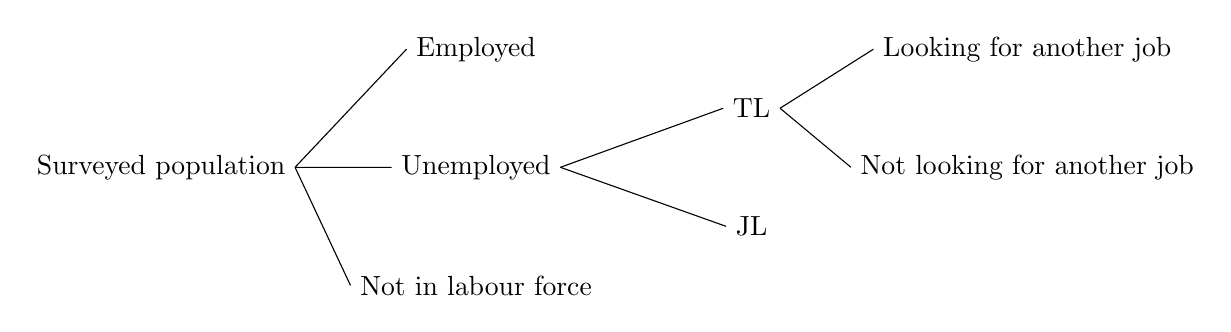
\begin{tikzpicture}[grow=right]
    \tikzset{level 1/.style={level distance = 4cm}}
    \tikzset{level 2/.style={level distance = 3.5cm}}
    \tikzset{level 3+/.style={level distance = 3cm}}
    \node{Surveyed population}
      child{node{Not in labour force}}
      child{node{Unemployed}
        child{node{JL}}
        child{node{TL}
          child{node{Not looking for another job}}
          child{node{Looking for another job}}
        }
      }
      child{node{Employed}}
    ;
  \end{tikzpicture}
  \caption{Tree structure of labour market status in CPS.}
  \subcaption*{TL = Temporary layoff, JL = Job-less unemployment (unemployment for any other reasons than temporary layoff). Definitions for the classifications are provided in the body text.}
  \label{cps_tree}
\end{figure}

Since CPS follows all individuals in selected households for across eight-month period, matching them across multiple monthly datasets enables one to conduct panel analysis, both at individual and household levels.
However, there is unfortunately no single variable that identifies either individuals or households across months, and I use a methodology and codes proposed by \cite{nekarda2009longitudinal} to overcome this issue.\footnote{While the codes are not provided for the paper by itself, Nekarda provided his codes for \cite{hall2018measuring}, and their replication package is available on the American Economic Association website and it includes Nekarda's codes.}
The main strategy is to use the household identifier variables \texttt{HRHHID} and \texttt{HRHHID2} to identify households and the person's line number variable \texttt{PULINENO} to identify individuals in a household.
However, there were changes in the specifications of the identifier variables across time, so technically slightly different matching strategies are adopted year by year.

Due to the nature of the survey, matching across multiple CPS datasets has limitations as follows.
First, as pointed out by \cite{pacas2015using}, there were changes in identifiers in June and September 1995 that break compatibility beyond those months.
Therefore, individual matchings are limited to within following three periods, and it is not possible to build links beyond each of them: before and including May 1995; June till August 1995; and September 1995 forward.
This paper will calculate the transition of labour market status in the adjacent two months, and due to this matching issue, job-finding rates for June and September 1995 are not available.
Second, in case of a surveyed household moving out in middle of the survey period, CPS do not follow that household in a new location.
Given a relationship between labour market status and geographical mobility, this may create a bias in longitudinal measurements \citep{nekarda2009longitudinal}.

Next, JOLTS reports monthly statistics on the demand side of the labour market in the US since December 2000.
It surveys a sample of around 21,000 companies in the US, compared to CPS that surveys randomly selected households.
This paper particularly uses the number of job openings and new hires each month from JOLTS.
It defines a job opening to be ``a specific position of employment to be filled at an establishment'', for which the employer is actively recruiting and is ready to start within 30 days.
On the other hand, a hire is defined in JOLTS as an addition to an establishment's payroll of both newly hired and rehired workers.
Therefore, importantly, one can interpret the hiring count in JOLTS as it includes both recruitment of new workers and recalls of previous employees who were on furlough.
Together with the unemployment level data from CPS, JOLTS is commonly used in the literature concerning the labour market tightness and job-finding rates.

\subsection{Alternative Datasets}

Although not analysed for this research, there are some alternative public datasets that are often used in the literature.
First, the Survey of Income and Program Participation (SIPP) is a commonly used longitudinal survey dataset along with CPS, which has advantages over CPS in that it allocates employer IDs to each individual, allowing researchers to follow the employers of workers before and after an unemployment spell, as practised by \cite{fujita2017recall}.
However, \cite{fujita2017recall} themselves point out an issue in some recalled workers being allocated a different employer ID to the previous one for the same employer.
Also, \cite{gertler2022temporary} suggest the existence of classification errors in types of unemployment, in that some permanent separation figures include temporary layoffs, leading to an overestimation of the proportion of JL unemployed workers who eventually returned to the last employer.
On the other hand, from CPS data, it is not possible to track individual TL workers whether they are actually returned to the last employer or build a job match with a new firm.
Some researchers, such as \cite{forsythe2022where}, focus instead on the industry of TL workers' new and old jobs and use as a proxy to be recalled if a worker works in the same industry to the previous job before the temporary layoff spell.

Second, a composite Help-Wanted Index developed by \cite{barnichon2010building} provides vacancy count estimates in the US labour market for the period before JOLTS data became available in December 2000.
The index is based on the traditional vacancy measure of the Conference Board Help-Wanted Index (HWI) which calculates the number of job advertisements in 51 major newspapers in the US.
However, as online job advertisements has become popular since mid-1990s, \cite{barnichon2010building} estimates the newspaper share by combining different datasets and weight the traditional HWI by that estimated share to build a composite index covering both print and online job advertisements.

\section{Descriptive Statistics}
\subsection{TL vs JL Unemployment}
Figure \ref{TL_share_out_of_U} shows the share of temporary layoff in all types of unemployment in the period between 1967 and 2019.
It shows the temporary layoff share has been consistent around 14\%, while it has fluctuated over business cycles.
Particularly, the share of TL seems to fluctuate somewhat countercyclically with surging TL share at the beginning of a recession, which is followed by a rapid drop that continues until after the end of a recession, and then the TL proportion recovers until the next recession.

\begin{figure}
  \centering
  \includegraphics[width=150mm]{TL_share_out_of_U.pdf}
  \caption{Share of temporary layoff in all types of unemployment}
  \subcaption*{Data source: CPS. Observation period is from January 1967 to December 2019. The solid line shows a quarter moving average of the monthly counts. All unemployment recorded on CPS is exclusively classified into one of the following types: job losers on layoff; job losers not on layoff; job leavers; reentrants to the labour force; and new entrants to the labour force. Shaded areas indicate recessions dated by NBER.}
  \label{TL_share_out_of_U}
\end{figure}

TL and JL unemployed workers appear to have different social characteristics as summarised in Table \ref{tlvsjl}.
First, we can see that TL workers were 18.3 and 9.6 percentage points more likely to be married and male, respectively.
For the unemployed, CPS defines the part-time workforce to be those who are on layoff from or looking for a part-time job, and similarly for the full-time workforce, and the table indicates TL workers had a 10.8 percentage points higher proportion of part-time workforce than JL workers.
The mean age of TL workers was 39.821, which was 6.597 years older than that of JL workers.
In terms of the highest education level received, the proportion of high school graduates was higher by 0.5 percentage points among TL workers, while it was 0.5 percentage points more prevalent to hold a bachelor degree among JL workers.

For the analysis of this table, monthly cross-section data are pooled onto a large dataset that covers the entire observation period.
Individuals are matched across months, and for those who reported as unemployed for multiple survey months, the response in the first survey month of unemployment is used to construct the table.
Also, Starting from May 2012, topcoding of age for 80 or over is introduced, and hence the table excludes those who are topcoded as such.

\begin{ltable}
  \begin{table}
\centering
\begin{talltblr}[         %% tabularray outer open
caption={Comparison of individual characteristics between TL and JL unemployed workers.\label{tlvsjl}},
note{}={\footnotesize{Data source: CPS. Observation period is from January 1994 to December 2019. For those who responded as unemployed for multiple times to the survey, the response in the first survey month of unemployment is used for the analysis. Individuals aged 80 or over are excluded. Part-time workforce indicates those who are on layoff from or looking for a part-time job instead of a full-time job. The base variable for the highest level of education indicator is not graduated from high school. Family income level classification can be found in the notes of Table \ref{familyinc_level}.}},
]                     %% tabularray outer close
{                     %% tabularray inner open
colspec={Q[]Q[]Q[]Q[]Q[]Q[]Q[]},
cell{1}{2}={c=2,}{halign=c,},
cell{1}{4}={c=2,}{halign=c,},
column{1}={halign=l,},
column{2}={halign=r,},
column{3}={halign=r,},
column{4}={halign=r,},
column{5}={halign=r,},
column{6}={halign=r,},
column{7}={halign=r,},
row{1}={halign=c,},
}                     %% tabularray inner close
\toprule
& JL workers &  & TL workers &  &  &  \\ \cmidrule[lr]{2-3}\cmidrule[lr]{4-5}
& Mean & Std. Dev. & Mean & Std. Dev. & Diff. in Means & Std. Error \\ \midrule %% TinyTableHeader
Married                                                 & \num{0.315}  & \num{0.465}  & \num{0.499}  & \num{0.500}  & \num{0.183}***  & \num{0.002} \\
Male                                                    & \num{0.504}  & \num{0.500}  & \num{0.600}  & \num{0.490}  & \num{0.096}***  & \num{0.002} \\
Part-time workforce                                     & \num{0.212}  & \num{0.409}  & \num{0.320}  & \num{0.467}  & \num{0.108}***  & \num{0.002} \\
Age                                                     & \num{33.224} & \num{14.504} & \num{39.821} & \num{14.816} & \num{6.597}***  & \num{0.055} \\
\Centerstack[l]{Graduated high school \\ but not holding a bachelor degree} & \num{0.041}  & \num{0.198}  & \num{0.045}  & \num{0.208}  & \num{0.005}***  & \num{0.001} \\
Holding a bachelor degree or above                      & \num{0.150}  & \num{0.357}  & \num{0.145}  & \num{0.352}  & \num{-0.005}*** & \num{0.001} \\
Family income level                                     & \num{8.423}  & \num{4.269}  & \num{9.419}  & \num{3.802}  & \num{0.997}***  & \num{0.014} \\
$N$                                                     & \num{466445} &               & \num{85052}  &               &                  &              \\
\bottomrule
\end{talltblr}
\end{table}

\end{ltable}

Next, Monthly CPS data do not include information for individual income unfortunately, and instead, family income of the last 12 months is recorded at levels as shown in Table \ref{familyinc_level}.

\begin{table}
  \centering
  \caption{Family income level classification.}
  \label{familyinc_level}
  \begin{tabular}{rl}
  \hline
  Level & Income               \\ \hline
  1     & Less than \$5,000    \\
  2     & \$5,000 to \$7,499   \\
  3     & \$7,500 to  \$9,999  \\
  4     & \$10,000 to \$12,499 \\
  5     & \$12,500 to \$14,999 \\
  6     & \$15,000 to \$19,999 \\
  7     & \$20,000 to \$24,999 \\
  8     & \$25,000 to \$29,999 \\
  9     & \$30,000 to \$34,999 \\
  10    & \$35,000 to \$39,999 \\
  11    & \$40,000 to \$49,999 \\
  12    & \$50,000 to \$59,999 \\
  13    & \$60,000 to \$74,999 \\
  14    & \$75,000 or more     \\ \hline
  \end{tabular}
  \subcaption*{In the raw CPS data, family income refers to combined income of all family members during the last 12 months, including both labour and non-labour incomes. Starting in October 2003, additional levels are introduced to classify the ranges \$75,000 to 99,999 and \$100,000 to 149,999. However, for this paper's analysis, those new levels are included in Level 14 for consistency with older data.}
\end{table}

Figure \ref{familyinc} shows the density of each family income level, comparing between TL and JL workers.
We can see that JL workers are more prevalent than TL workers are for family income levels of 5 or below, while at Level 6, a range between \$15,000 and 19,999, there was almost no difference between the two types of unemployment.
On the other hand, for the level 6 or higher, TL workers marked higher densities, and the difference between the two types of unemployment enlarges as the income level becomes higher.
This result is, to some extent, comparable with the finding of \cite{nekoei2020seven}, who analysed Austrian unemployment registers and found a peak of TL rate around 80th percentile of the wage distribution.
The authors give a hypothesis that TL workers are such that it is more difficult for employers to replace with, compared to permanent separation in which case firms have to spend hiring costs to fill vacancies.
If this hypothesis is true, TL workers' (previous) wage should be higher than JL workers', and family income as a proxy should exhibit the same tendency, as shown in Figure \ref{familyinc}.

\begin{figure}
  \centering
  \includegraphics[width=150mm]{familyinc.pdf}
  \caption{Density of TL/JL unemployed workers by family income level}
  \subcaption*{Data source: CPS. Observation period is from January 1994 to December 2019. Family income level classification refers to Table \ref{familyinc_level}.}
  \label{familyinc}
\end{figure}

\subsection{TL Unemployed Workers on Search vs Not on Search for Another Job}
I also compare the characteristics of TL unemployed workers who are looking for an alternative job and those who are not.
First, Figure \ref{search_TL_share} shows the proportion of TL unemployed workers who responded as they have been looking for work during the last 4 weeks.
It shows a clear countercyclical pattern of the movement in business cycles, with the proportion surged from 34.5\% to 39\% during the 2001 Dot Com recession, after which the figure constantly decreased to 33\% just before the financial recession, followed by another surge to 45\% and a subsequent decreasing trend to 25\% before the outbreak of the pandemic.
\begin{figure}
  \centering
  \includegraphics[width=150mm]{search_TL_share.pdf}
  \caption{Share of TL workers who are looking for an alternative job in all TL workers}
  \subcaption*{Data source: CPS. Observation period is from January 1994 to December 2019. The black solid line indicates the 12-month moving average of the monthly proportion values. Shaded areas denote recessions dated by NBER.}
  \label{search_TL_share}
\end{figure}

In order to investigate factors that determine whether furloughed workers look for an alternative job or not, a set of logistic regression models are estimated using pooled CPS data.
The baseline model is a logistic regression of an indicator for looking for another job on holding a return date:
\begin{equation}
  \E[Y_{it}|X_{it}] = \Lambda(\beta_0 + \beta_1 X_{it}),
\end{equation}
where $\Lambda(z) \equiv \exp(z) / {1 + \exp(z)}$ and $Y_{it} = I(\text{looking for another job}_{it})$ and $X_{it} = I(\text{holding a return date}_{it})$ for the individual $i$ at time $t$.
The estimation results are reported in average partial effects in Column (1) of Table \ref{log_reg_res}.
Next, year fixed-effects are added to the baseline model, whose results are shown in Column (2).
For the remaining four models, different covariates are introduced, among which layoff duration is in weeks, age in years, and the others dummy indicators for the individual $i$ at time $t$, with and without time fixed-effects.

The dummy variable for holding a return date was the largest in the absolute size of average partial effect among the regressors in all six models of at least -0.155.
Note due to the definition of temporary layoff, those who do not hold a return date have to be given an indication to be recalled by their last employers.
Therefore, the regression results indicate holding a return date is associated with at least 15.5\% lower probability that the individual is looking for another job, compared to when s/he is given only an indication and does not hold a specific date to return.
Comparing the estimates across all six columns, the estimated size shrank as covariates and/or year fixed effects were added to the model.
This would suggest that whether for an unemployed worker to hold a return date or not is correlated with social factors and/or the timing of layoff, and not controlling for those determinants could end up in suffering from variable omitted bias.

Furthermore, layoff duration was positively associated with the probability of job search during temporary layoff with an increase by 0.4\% for an additional week of the unemployment spell.
Also, being younger, male, and in full-time workforce were the factors that increase the probability of conducting job search.
In terms of the highest education received, having graduated from high school is positively associated with the probability, while holding a bachelor degree negatively associated, with the latter being larger in the absolute size of the average partial effect.

For the analysis, individual fixed effects estimators would reduce omitted variable bias by eliminating unobserved, time-invariant heterogeneity across individuals through demeaning.
However, estimating an individual fixed effect model requires individuals to appear in a dataset at least in two periods, which in this case means only the TL unemployed workers whose duration was longer than two months of the CPS survey period are considered.
Over the observation period between 1994 and 2019, there were 26,809 of such individuals, which accounts only for 31.52\% of the total workers who experienced temporary layoff.
Furthermore, layoff duration would have a correlation with other social characteristics of TL workers.
Therefore, an individual fixed effects model would not be appropriate to represent the entire TL population and is omitted from the analysis.

\begin{ltable}
  \begin{table}
\centering
\begin{talltblr}[         %% tabularray outer open
caption={Results of logistic regressions.\label{log_reg_res}},
note{}={+ p \num{< 0.1}, * p \num{< 0.05}, ** p \num{< 0.01}, *** p \num{< 0.001}},
note{ }={\footnotesize{Data source: CPS. Observation period is from January 1994 to December 2019. Average partial effects are reported with heteroscedasticity-robust standard errors in brackets. Individuals aged 80 or over are excluded. Part-time workforce indicates those who are on layoff from or looking for a part-time job instead of a full-time job. The base variable for the highest level of education indicator is not graduated from high school.}},
]                     %% tabularray outer close
{                     %% tabularray inner open
colspec={Q[]Q[]Q[]Q[]Q[]Q[]Q[]},
column{1}={halign=l,},
column{2}={halign=c,},
column{3}={halign=c,},
column{4}={halign=c,},
column{5}={halign=c,},
column{6}={halign=c,},
column{7}={halign=c,},
hline{16}={1,2,3,4,5,6,7}{solid, 0.05em, black},
}                     %% tabularray inner close
\toprule
& (1) & (2) & (3) & (4) & (5) & (6) \\ \midrule %% TinyTableHeader
Holding a return date                                        & \num{-0.180}*** & \num{-0.175}*** & \num{-0.171}*** & \num{-0.167}*** & \num{-0.157}*** & \num{-0.154}*** \\
& (\num{0.002})   & (\num{0.003})   & (\num{0.002})   & (\num{0.002})   & (\num{0.002})   & (\num{0.002})   \\
Layoff duration (weeks)                                      &                  &                  & \num{0.005}***  & \num{0.004}***  & \num{0.004}***  & \num{0.004}***  \\
&                  &                  & (\num{0.000})   & (\num{0.000})   & (\num{0.000})   & (\num{0.000})   \\
Age                                                          &                  &                  &                  &                  & \num{-0.003}*** & \num{-0.003}*** \\
&                  &                  &                  &                  & (\num{0.000})   & (\num{0.000})   \\
Holding a bachelor degree or above                           &                  &                  &                  &                  & \num{-0.015}*** & \num{-0.012}**  \\
&                  &                  &                  &                  & (\num{0.004})   & (\num{0.004})   \\
\Centerstack[l]{Graduated from high school \\ but not holding a bachelor degree} &                  &                  &                  &                  & \num{-0.057}*** & \num{-0.053}*** \\
&                  &                  &                  &                  & (\num{0.008})   & (\num{0.008})   \\
Male                                                         &                  &                  &                  &                  & \num{0.039}***  & \num{0.037}***  \\
&                  &                  &                  &                  & (\num{0.003})   & (\num{0.003})   \\
Part-time workforce                                          &                  &                  &                  &                  & \num{-0.122}*** & \num{-0.120}*** \\
&                  &                  &                  &                  & (\num{0.003})   & (\num{0.003})   \\
Number of observations                                       & \num{148433}    & \num{148433}    & \num{148433}    & \num{148433}    & \num{148433}    & \num{148433}    \\
Year FE                                                      &                  & X                &                  & X                &                  & X                \\
AIC                                                          & \num{190406.5}  & \num{189235.6}  & \num{188722.4}  & \num{187699.3}  & \num{184220.2}  & \num{183474.3}  \\
\bottomrule
\end{talltblr}
\end{table}

\end{ltable}

\subsection{Job-finding Rates by Types of Unemployment}
A job-finding rate is the probability that an unemployed worker finds a job in a given period.
While the literature proposes various ways to estimate this probability and indeed the main analysis of this paper adopts an alternative methodology as discussed below, here I calculate it by tracking the transitions of individual labour market status recorded in longitudinally matched micro-level CPS data.
In this way, the job-finding rates are calculated as follows: first, match the individuals who were unemployed in the previous month in the current month dataset, and classify them whether they have become employed or not.
Then, the job-finding rates among the unemployed in month $t$, $F_t$, is the ratio of the number of workers who were unemployed in the last month $t - 1$ but have become employed in the current month $t$, $N(U_{t-1}E_t)$, to the number of the unemployed in the last month, $N(U_{t-1})$.
Therefore, the job-finding rate is $F_t = \dfrac{N(U_{t-1}E_t)}{N(U_{t-1})}$.

A similar approach is taken by \cite{hall2018measuring} who estimated job-finding rates for heterogeneous workers in periods of different lengths.
As they suggest, an advantage of this method is the capability for computing the probability for different types of unemployment.
For example, I can estimate the job-finding rate for TL workers who conduct job search in the previous month by calculating the employment probability only among those TL workers.
Also, despite not being used for this paper's analysis, job-finding rates in a various period, rather than in one month, can be calculated by matching individuals over a longer time period.

Figure \ref{finding_rates_by_search} shows the movements of job-finding rates for all unemployment types combined, as well as by whether searching for a new job or not (the unemployed not searching for a new job are some of those on temporary layoff).
The blue line indicates the job-finding rate for those not looking for a new job and the red line the population of ``on-unemployment search''.
On the other hand, the green line is for all unemployed workers, which is the weighted average of the other two rates.
The red and green lines show a procyclical pattern with sharp falls during recessions followed by gradual recoveries.
In contrast, the blue line, non-searching TL workers, implies a more zigzagging movement across time and was consistently higher than the other two lines at around 50\%, meaning that around half of the non-searching TL workers went back to employment in the following month.

\begin{figure}
  \centering
  \includegraphics[width=150mm]{finding_rates_by_search.pdf}
  \caption{job-finding rates for the unemployed by whether searching for a new job or not}
  \subcaption*{Data source: CPS. Observation period is from October 1995 to December 2019. Yearly moving average of the monthly data is shown. Job-finding rate for the unemployed looking for a new job is the probability of those workers becoming employed in the following month. Similar for that for TL workers not looking for another job, and the rate for all unemployed is the weighted average of the two. Shaded areas indicate recessions dated by NBER.}
  \label{finding_rates_by_search}
\end{figure}

Next, Figure \ref{finding_rates_JLTL} shows the finding rates for groups of unemployment aggregated at different levels.
The red line shows the rate among all JL workers, while the light green among all TL workers.
TL workers are further divided according to whether they conduct job search or not, indicated by light blue and purple lines, respectively.
Across the 24-year period, it was consistently the case that the job-finding rate was the highest among non-searching TL workers, followed by searching TL workers and JL workers, and the movements of the three types were similar from a holistic viewpoint.
Particularly, lower job-finding rates among TL workers who were searching for another job than among not searching implies that layoff spell length may be due to each worker's characteristics, of which some were explored above, rather than a consequence of whether to conduct job search or not itself.

\begin{figure}
  \centering
  \includegraphics[width=150mm]{finding_rates_JLTL.pdf}
  \caption{Comparison of job-finding rates for different types of unemployed workers}
  \subcaption*{Data source: CPS. Observation period is from October 1995 to December 2019. Yearly moving average of the monthly data is shown. Job-finding rate for the JL unemployed workers is the probability of those becoming employed in the following month. Similar for the other three job-finding rates. Shaded areas indicate recessions dated by NBER.}
  \label{finding_rates_JLTL}
\end{figure}

Finally, I compare the job-finding rates among all unemployment types under this CPS transition-based strategy with another method based on JOLTS' new hiring counts.
This strategy estimates the job-finding rates as a ratio of new hiring counts from JOLTS to the level of unemployment from CPS, which this paper adopts for the main analysis below, following the popularity among the literature.
In Figure \ref{finding_rates_benchmark}, the light blue line shows the original CPS transition-based estimates, while the red line JOLTS new hiring counts divided by the level of unemployment from CPS.
For the same estimation target of job-finding rates, the two estimation strategies resulted in a large difference in volatility.
This difference should be due to the nature of those two surveys, and because JOLTS does not have information on some labour market statistics, such as the unemployment level or matching efficiency \citep{hall2018measuring}, it would not be possible to fully examine the difference between CPS and JOLTS markets.
Following the majority of the literature, the main analysis of the paper below will employ the JOLTS-based job-finding rates.

\begin{figure}
  \centering
  \includegraphics[width=150mm]{finding_rates_benchmark.pdf}
  \caption{Comparison of estimated finding rates based on JOLTS hiring level vs. labour market transitions in CPS}
  \subcaption*{Data source: CPS and JOLTS. Observation period is from December 2000 to December 2019. Job-finding rates are estimated based on (1) JOLTS hiring level divided by CPS unemployment level (2) probability of an unemployed worker being employed in the following month as recorded in raw CPS data. Shaded areas indicate recessions dated by NBER.}
  \label{finding_rates_benchmark}
\end{figure}

\section{Methodology\label{methodology}}

\subsection{Estimating a Basic Matching Function}
A matching function in the labour market relates the level of unemployment and the number of vacancies in the market to the level of new hires in a given period.
Let $M_t, U_t$, and $V_t$ be the levels of matching, unemployment, and vacancy at time $t$, respectively.
Then, a general matching function $m(\cdot)$ is expressed mathematically as
\begin{align}
  m: \mathbb{R}_+^2 \to \mathbb{R}_+, M_t &= m(U_t, V_t),
\end{align}
for which it is assumed to be increasing in both inputs, concave, no unemployment or vacancy resulting in no new matchings, i.e., $m(0, V_t) = m(U_t, 0) = 0$, and the number of new matches no larger than the level of unemployment or vacancy, i.e., $m(U_t, V_t) \leq \min\{U_t, V_t\}$.
As like the majority of the matching function literature, I impose a constant returns to scale Cobb-Douglas functional form on this function, so that
\begin{align}
  M_t = A_tU^{1-\eta}V_t^\eta,
\end{align}
where $A_t$ and $\eta$ are parameters.
Dividing both sides by $U_t$ gives
\begin{equation}
  \frac{M_t}{U_t} = A_t\qty(\frac{V_t}{U_t})^\eta.
\end{equation}
This indicates the matching function can also be interpreted as the relationship between a job-finding rate and a market tightness measure, which, in my way, are calculated as $F_t = \dfrac{M_t}{U_t}$ and $\Theta_t = \dfrac{V_t}{U_t}$.
Therefore, the alternative form of the matching function links the level of market tightness to a job-finding rate as
\begin{equation}
  F_t = A_t\Theta_t^\eta.
\end{equation}
Taking the log of both sides gives a linear version of this formula,
\begin{equation}
  f_t = \eta\theta_t + a_t,
\end{equation}
where $f_t = \log F_t, \theta_t = \log\Theta_t$, and $a_t = \log A_t$, which is convenient for empirical estimation.
For most literature in estimating an empirical matching function, $\eta$ and $a_t$ are the parameters of interest because the former indicates the elasticity of the job-finding rate with respect to labour market tightness and the latter the matching efficiency of the market.
Also, following many papers studying the US labour market, I use the unemployment level $U_t$ from CPS and hiring and vacancy levels $M_t$ and $V_t$ from JOLTS.
Furthermore, following \cite{borowczyk-martins2013accounting}, I assume the efficiency parameter $a_t$ is a composite of a constant $\mu$, a monthly seasonal dummy $\tau$, and an unobserved component $\varepsilon_t$.
Therefore, the estimation expression will be
\begin{equation}\label{matching_function_formula}
  f_t = \mu + \eta\theta_t + \tau + \varepsilon_t.
\end{equation}

\subsection{Heterogeneous Unemployed Workers}
As an extension to this basic Cobb-Douglas matching function, I introduce the heterogeneity in unemployed workers, such that some workers are on temporary layoff and either searching for a new job or not, while the others are on jobless unemployment, as described in the previous section.
First, I distinguish unemployment types according to whether workers are searching for a new job or not.
The unemployed who are not searching are some of the TL workers, whose level hereafter is denoted by $TL_{nosearch}$, while those looking for a new job is the sum of the remaining TL workers and all JL workers, i.e., $U_{search} = JL + TL_{search}$.
Note that sum of the populations of searching unemployed workers and non-searching (TL) unemployed workers will be the entire unemployment, i.e., $U = U_{search} + TL_{nosearch}$.

Assume, in an extended model, each level of the searching and non-searching unemployed workers matters for determining the number of new job-matches in addition to the level of vacancies.
Then, the matching function will be
\begin{equation}
  m: \mathbb{R}_+^3 \to \mathbb{R}_+, M_t = m(U_{\text{search, }t}, TL_{\text{nosearch, }t}, V_t).
\end{equation}
Here, I impose a constant returns to scale Cobb-Douglas functional form as before, so that
\begin{equation}
  M_t = A_tU_{\text{search, }t}^{1 - \alpha - \eta}TL_{\text{nosearch, }t}^\alpha V_t^\eta,
\end{equation}
where $\alpha$ and $\eta$ are parameters.
Dividing both sides by $U_{\text{search, }t}$ gives
\begin{equation}
  \frac{M_t}{U_{\text{search, }t}} = A_t\qty(\frac{TL_{\text{nosearch, }t}}{U_{\text{search, }t}})^\alpha\qty(\frac{V_t}{U_{\text{search, }t}})^\eta.
\end{equation}
By taking a log of both sides,
\begin{equation}
  \log\qty(\frac{M_t}{U_{\text{search, }t}}) = \eta\log\qty(\frac{V_t}{U_{\text{search, }t}}) + \alpha\log\qty(\frac{TL_{\text{nosearch, }t}}{U_{\text{search, }t}}) + a_t,
\end{equation}
where $a_t = \log A_t$ as before.
Similar to the baseline model described above, assume $a_t = \mu + \tau + \varepsilon_t$, so that
\begin{equation} \label{matching_function_formula_by_search}
  \log\qty(\frac{M_t}{U_{\text{search, }t}}) = \mu + \eta\log\qty(\frac{V_t}{U_{\text{search, }t}}) + \alpha\log\qty(\frac{TL_{\text{nosearch, }t}}{U_{\text{search, }t}}) + \tau + \varepsilon_t.
\end{equation}
I hereafter call this extended model as the ``search/non-search split model''.

A motivation for this extension is to separate out the non-searching TL workers from the labour market because their non-searching behaviour would not affect the competitiveness regarding job-finding process of the other unemployed workers.
Then, $\eta$ in this equation will have a different interpretation than the one in Equation \ref{matching_function_formula}:
the original $\eta$ in Equation \ref{matching_function_formula} implies an elasticity of job-finding rate, $M_t / U_t$, with respect to the market tightness measured as $V_t / U_t$;
the new $\eta$ is a partial elasticity of the ratio $M_t / U_{\text{search, }t}$ with respect to the number of vacancies per searching unemployed worker, $V_t / U_{\text{search, }t}$.
Given the difference, I argue from a theoretical perspective that this new $\eta$ in Equation \ref{matching_function_formula_by_search} better represents the frictions faced by unemployed workers and firms seeking for establishing a new match.
In Equation \ref{matching_function_formula_by_search}, the number of new matchings $M_t$, which includes both new hires and recalling of previous workers in JOLTS measure, is explained by the level of vacancies as well as the number of non-searching TL workers.
Since recalling of TL workers is a cost-free process for both workers and firms, this friction-less component of job matches should be excluded from measuring a cost of job search.

\subsection{Endogeneity Issue in Estimating a Matching Function}
Estimating Equation \ref{matching_function_formula} by OLS is the most basic and common strategy in the literature.
However, \cite{borowczyk-martins2013accounting} argue that it suffers from an endogeneity issue.
They point out the job-finding rate $f_t$ is clearly correlated with the efficiency parameter $a_t$ (or $\varepsilon_t$) because as the labour market gains efficiency in matching between workers and employers, job-finding rate would increase not only directly, but also indirectly through firms posting more vacancies.

In order to resolve the endogeneity issue that was raised above, I incorporate an instrumental variable approach proposed by \cite{yashiv2000determinants} (which was used by \cite{borowczyk-martins2013accounting} to compare with their proposing strategy of GMM to estimate under an assumption of $\varepsilon_t$ in Equation \ref{matching_function_formula} following an ARMA process).
After taking a first difference to cater for nonstationarity, \cite{yashiv2000determinants} uses up to five lags of the (log of) market tightness measure $\theta_{t - \ell}, \ell = \{2, 3, 4, 5\}$ as instruments for the first difference of market tightness $\Delta\theta_t = \theta_t - \theta_{t - 1}$, and I follow this strategy in my estimation.
\cite{yashiv2000determinants} chooses the instruments as such based on Monte Carlo simulation results suggesting a preference for parsimony in selecting instruments, while at the same time the relevance condition needs to be satisfied.
Implementing those instruments gives us a consistent estimate of $\eta$, given $\varepsilon_t$ is a random walk.

In terms of the proposed extended matching function model of Equation \ref{matching_function_formula_by_search}, the first difference of $\log\qty(\dfrac{V_t}{U_{\text{search, }t}})$ is treated as endogenous and instrumented by its second till fifth lags, while $\log\qty(\dfrac{TL_{\text{nosearch, }t}}{U_{\text{search, }t}})$ is treated as an exogenous variable.
% TODO: explain the source of endogeneity / reasons for IV


\section{Results}

\subsection{Matching Function Estimates for the Baseline and Extended ``Search/no-search Split'' Models}
I first estimated the baseline matching function as well as the extended one that splits out some TL workers not on search for an alternative job from the entire unemployed population.
The regression estimation results are shown in Table \ref{matching_fn}.
Columns (1) and (2) show the estimation results for both models by OLS.
The elasticity of job-finding with respect to the market tightness, $\eta$, is clearly different according to the treatment of the heterogeneity in unemployment.
In the baseline model in Column (1), the elasticity was estimated to be 0.693, while Column (2) shows the estimate for the extended ``search/non-search split'' model of 0.551.
This means that, based on the extended model, one per cent increase in the alternative market tightness measure, $V_t / U_{\text{search, }t}$, will result in 0.551 per cent increase in the job-finding rate among the unemployed on search for a new job, given the ratio of non-searching TL to the other unemployed workers does not change.
This difference would imply that, based on an assumption of separate labour markets for non-searching TL workers and the other unemployed workers, the elasticity of job-finding with respect to the market tightness for the unemployed who are actually looking for a new job should be lower than the baseline model by 0.142.
Also, an estimate for $\alpha$ in Column (2) was 0.439 and statistically significant to be non-zero, meaning that a relative increase in non-searching TL workers is also related to an increase in matchings (divided by the searching unemployed population).
Plus, a slight increase in $R^2$ from 0.918 to 0.944 (or equivalently, a reduction in RMSE) implies that a separate treatment of non-searching TL workers improves the model capture.

\begin{table}
\centering
\begin{talltblr}[         %% tabularray outer open
caption={Matching function estimation: baseline vs split in unemployment depending on searching or not\label{matching_fn}},
note{}={+ p < 0.1, * p < 0.05, ** p < 0.01, *** p < 0.001},
note{ }={\footnotesize{Data source: CPS and JOLTS. Observation period is from December 2000 to December 2019. The odd numbered columns show estimates for the baseline model, while the even numbered for the extended model treating non-searching TL workers differently. Month dummies are included in the estimation. Heteroscedasticity-robust standard errors are reported in parentheses. Instruments for Columns (5) and (6) are up to 5 lags of the corresponding endogenous variable.}},
]                     %% tabularray outer close
{                     %% tabularray inner open
colspec={Q[]Q[]Q[]Q[]Q[]Q[]Q[]},
cell{1}{2}={c=2,}{halign=c,},
cell{1}{4}={c=2,}{halign=c,},
cell{1}{6}={c=2,}{halign=c,},
column{1}={halign=l,},
column{2}={halign=c,},
column{3}={halign=c,},
column{4}={halign=c,},
column{5}={halign=c,},
column{6}={halign=c,},
column{7}={halign=c,},
hline{9}={1,2,3,4,5,6,7}{solid, 0.05em, black},
}                     %% tabularray inner close
\toprule
& OLS &  & OLS in FD &  & IV in FD &  \\ \cmidrule[lr]{2-3}\cmidrule[lr]{4-5}\cmidrule[lr]{6-7}
& (1) & (2) & (3) & (4) & (5) & (6) \\ \midrule %% TinyTableHeader
(Intercept)               & -0.157*** & 0.725*** &          &          &             &             \\
& (0.029)   & (0.082)  &          &          &             &             \\
$\eta$                   & 0.693***  & 0.551*** & 0.314*** & 0.313*** & 0.504***    & 0.527***    \\
& (0.012)   & (0.020)  & (0.044)  & (0.044)  & (0.136)     & (0.133)     \\
$\alpha$                 &           & 0.439*** &          & 0.010    &             & -0.004      \\
&           & (0.041)  &          & (0.025)  &             & (0.026)     \\
Sargan test               &           &          &          &          & 11.9$^{**}$ & 11.9$^{**}$ \\
($p$-value)               &           &          &          &          & (0.0078)    & (0.0025)    \\
First stage $F$ statistic &           &          &          &          & 9.68        & 10.2        \\
Num.Obs.                  & 229       & 229      & 228      & 228      & 224         & 224         \\
R2                        & 0.918     & 0.944    & 0.900    & 0.894    & 0.890       & 0.880       \\
RMSE                      & 0.12      & 0.10     & 0.05     & 0.05     & 0.05        & 0.05        \\
\bottomrule
\end{talltblr}
\end{table}


Next, Columns (3) and (4) show the estimates of both models in first differences, following the literature that might worry the existence of unit roots in the job-finding rates and/or the market tightness giving spurious estimates of the elasticity.
Estimates for $\eta$ were almost the same at 0.314 and 0.313 for the baseline and extended models, respectively, and that for $\alpha$ in the extended model in Column (4) resulted to be statistically non-significant.
Therefore, in the first-differenced term, I can argue that some TL workers not looking for an alternative job did not affect the job-finding of the other unemployed workers on search for a new job.

To investigate the stationarity of all variables in Equations \ref{matching_function_formula} and \ref{matching_function_formula_by_search}, I executed an augmented Dicky-Fuller test with a drift term and lags of up to 30 chosen based on AIC.
It turned out only $\log\qty(\dfrac{TL_{\text{nosearch, }t}}{U_{\text{search, }t}})$ rejected the null hypothesis, implying the unit root existence in all other variables.
This may concern about a spurious correlation in the OLS estimates in Columns (1) and (2), and indeed, first-differenced estimates in Columns (3) and (4) are significantly different.
That being said, \cite{borowczyk-martins2013accounting}, who computed the baseline model of this paper, interpret as a reflection of different biases, rather than a result of a spurious correlation between the two non-stationary series as this is a structural estimation.

Finally, Columns (5) and (6) show an attempt to handle possible endogeneity in the matching function equations using the instrumental variable method in first-differenced variables with the second till fifth lags of market tightness as instruments.
Column (5) is the estimation results for the baseline model.
Here, the first difference in the market tightness, $\Delta\theta_t = \Delta\log\qty(\dfrac{V_t}{U_t})$ is treated to be endogenous, and the elasticity was estimated to be 0.504, sitting in the middle of the OLS and first-differenced OLS estimates.
On the other hand, Column (6) is for the extended model with a first difference $\log\qty(\dfrac{V_t}{U_{\text{search, }t}})$ instrumented by lags of the original values.
The elasticity estimates are again very similar across both models with 0.504 and 0.517, and also the estimated value of $\alpha$, a coefficient for $\log\qty(\dfrac{TL_{\text{nosearch, }t}}{U_{\text{search, }t}})$ in the extended model was not statistically significant.
This implies the heterogeneity in the unemployment that some TL workers are not on search did not give a statistically significant impact in estimating the job-finding rates.
In terms of the validity of the instruments, the first stage $F$ statistic was 9.68 and 10.2 for the baseline and extended models, respectively.
Compared to the rule-of-thumb value of 10 proposed by \cite{staiger1997instrumental}, I would generously argue that the relevance condition is satisfied.
In contrast, it is questionable whether the instruments satisfied the exclusion requirement or not, according to the Sargan test which rejected the null hypothesis at 1 per cent significance level for both models.

My elasticity estimates for the baseline model in Columns (1), (3), and (5) of Table \ref{matching_fn} are comparable with the findings by \cite{borowczyk-martins2013accounting} as I followed their estimation strategies and used the same data, but for a wider observation period up to December 2019 than theirs up to January 2012.
First, their OLS estimate is 0.842, significantly higher than mine of 0.693 in Column (1), for which I believe my lower estimate is simply a reflection of the low market matching efficiency trend after the 2008 recession that continued until the end of my observation period.
On the other hand, my first-differenced estimates of 0.314 by OLS in Column (3) and 0.504 by the instrumental variable method in Column (5) resulted in similar values to theirs of 0.331 and 0.412, respectively.
This may imply that, in spite of the low matching efficiency trend in 2010s, changes in the market tightness measure between two adjacent periods affected the job-finding rates in a similar size as before.

\subsection{Matching Function at Different Aggregation Levels of Unemployment Types}
To compare the matching function estimates with heterogeneous unemployment at different aggregation levels, I consider following two additional models.
First, I separated the unemployed workers into either on temporary layoff or on jobless unemployment (hereafter referred as ``JL/TL split'').
In this case, the matching function will be
\begin{equation}
  M_t = A_tJL_t^{1 - \alpha - \eta}TL_t^\alpha V_t^\eta
\end{equation}
by imposing a constant returns to scale Cobb-Douglas functional form as before.
This is again taken a log to transform into a linear form:
\begin{align}
  \log\qty(\frac{M_t}{JL_t}) &= \eta\log\qty(\frac{V_t}{JL_t}) + \alpha\log\qty(\frac{TL_t}{JL_t}) + a_t \\
                             &= \mu + \eta\log\qty(\frac{V_t}{JL_t}) + \alpha\log\qty(\frac{TL_t}{JL_t}) + \tau + \varepsilon_t. \label{matching_function_formula_JLTL}
\end{align}
Second, a matching function recognises the heterogeneity in unemployment by classifying them into JL, TL on search, or TL not on search.
I call this model the ``three-way split model'' hereafter.
Then, the function is expressed as
\begin{equation}
  M_t = A_tJL_t^{1 - \alpha - \beta - \eta}TL_{search,t}^\alpha TL_{\text{nosearch, }t}^\beta V_t^\eta,
\end{equation}
with its log form
\begin{align}
  \log\qty(\frac{M_t}{JL_t}) &= \eta\log\qty(\frac{V_t}{JL_t}) + \alpha\log\qty(\frac{TL_{\text{search, }t}}{JL_t}) + \beta\log\qty(\frac{TL_{\text{nosearch, }t}}{JL_t}) + a_t \\
                             &= \mu + \eta\log\qty(\frac{V_t}{JL_t}) + \alpha\log\qty(\frac{TL_{\text{search, }t}}{JL_t}) + \beta\log\qty(\frac{TL_{\text{nosearch, }t}}{JL_t}) + \tau + \varepsilon_t \label{matching_function_formula_JLTLs}
\end{align}
to be estimated.
As before, I estimated Equations \ref{matching_function_formula_JLTL} (the ``JL/TL split'') and \ref{matching_function_formula_JLTLs} (the ``three-way split'') by OLS, by OLS in first difference, and by the instrumental variable method in first difference with treating $\log\qty(\dfrac{V_t}{JL_t})$ as endogenous instrumented by up to the fifth lags of itself.
$\log\qty(\dfrac{TL_t}{JL_t})$ in Equation \ref{matching_function_formula_JLTL} and $\log\qty(\dfrac{TL_{\text{search, }t}}{JL_t})$ and $\log\qty(\frac{TL_{\text{nosearch, }t}}{JL_t})$ in Equation \ref{matching_function_formula_JLTLs} are treated as exogenous variables.

The estimation results are shown in Table \ref{matching_fn_compare}.
Odd numbered columns show the estimates of the JL/TL split model, corresponding to Equation \ref{matching_function_formula_JLTL}.
In Column (1), the elasticity estimate of 0.597 is lower than the baseline model of 0.693, while in Columns (3) and (5) when the model takes the first difference and instrumented by the lags of market tightness, the estimated elasticity eventually became similar to the baseline model with 0.316 in Column (3) and 0.523 in Column (5), compared with 0.314 and 0.504, given the size of standard errors.

\begin{table}
\centering
\begin{talltblr}[         %% tabularray outer open
caption={Matching function estimation: alternative splits in unemployment\label{matching_fn_compare}},
note{}={+ p < 0.1, * p < 0.05, ** p < 0.01, *** p < 0.001},
note{ }={\footnotesize{Data source: CPS and JOLTS. Observation period is from December 2000 to December 2019. The odd numbered columns show estimates for the JL/TL split model, while the even numbered for the three-way split model. Month dummies are included in the estimation. Heteroscedasticity-robust standard errors are reported in parentheses. Instruments for Columns (5) and (6) are up to 5 lags of the corresponding endogeneous variable.}},
]                     %% tabularray outer close
{                     %% tabularray inner open
colspec={Q[]Q[]Q[]Q[]Q[]Q[]Q[]},
cell{1}{2}={c=2,}{halign=c,},
cell{1}{4}={c=2,}{halign=c,},
cell{1}{6}={c=2,}{halign=c,},
column{1}={halign=l,},
column{2}={halign=c,},
column{3}={halign=c,},
column{4}={halign=c,},
column{5}={halign=c,},
column{6}={halign=c,},
column{7}={halign=c,},
hline{11}={1,2,3,4,5,6,7}{solid, 0.05em, black},
}                     %% tabularray inner close
\toprule
& OLS &  & OLS in FD &  & IV in FD &  \\ \cmidrule[lr]{2-3}\cmidrule[lr]{4-5}\cmidrule[lr]{6-7}
& (1) & (2) & (3) & (4) & (5) & (6) \\ \midrule %% TinyTableHeader
(Intercept)               & 0.660*** & 1.120*** &          &          &             &             \\
& (0.054)  & (0.070)  &          &          &             &             \\
\eta                     & 0.597*** & 0.661*** & 0.316*** & 0.320*** & 0.523***    & 0.533***    \\
& (0.015)  & (0.026)  & (0.044)  & (0.044)  & (0.134)     & (0.132)     \\
\alpha                   & 0.512*** & 0.352*** & 0.049    & 0.059**  & 0.029       & 0.055*      \\
& (0.035)  & (0.043)  & (0.031)  & (0.021)  & (0.033)     & (0.023)     \\
\beta                    &          & 0.160**  &          & 0.005    &             & -0.010      \\
&          & (0.058)  &          & (0.025)  &             & (0.027)     \\
Sargan test               &          &          &          &          & 12.3$^{**}$ & 11.5$^{**}$ \\
($p$-value)               &          &          &          &          & (0.0065)    & (0.0093)    \\
First stage $F$-statistic &          &          &          &          & 10.1        & 10.1        \\
Num.Obs.                  & 229      & 229      & 228      & 228      & 224         & 224         \\
R2                        & 0.950    & 0.956    & 0.890    & 0.892    & 0.877       & 0.878       \\
RMSE                      & 0.09     & 0.09     & 0.05     & 0.05     & 0.05        & 0.05        \\
\bottomrule
\end{talltblr}
\end{table}


On the other hand, for the three-way split model of Equation \ref{matching_function_formula_JLTLs}, the OLS estimate shown in Column (2) was 0.661, which is closer to the baseline model estimate.
Similar to the two previous models of heterogeneous unemployment, taking first differences appeared to eliminate the elasticity difference arising from incorporating the heterogeneity in unemployed workers, with 0.320 compared to the baseline estimate of 0.314.
Meanwhile, using the instrumental variable method in Column (6) gave an estimated elasticity of 0.533, which is slightly higher than the baseline estimate of 0.504 as well as the two other heterogeneous unemployment models.
In terms of the validity of the instruments, the relevance condition seems to be satisfied according to the first stage $F$ statistic of 10.1 for both models in Columns (5) and (6), whereas the satisfaction of the exclusion requirement is questionable based on the Sargan test results, similar to the estimates in Table \ref{matching_fn}.

\subsection{Estimated Matching Efficiencies}
While the above discussions are about the estimated results of job-finding elasticities, estimation of a matching function also gives a numerical measure of market efficiencies.
As I defined the market efficiency to be a composite of a constant term, a monthly seasonal dummy, and an unobserved component, the residuals of the estimation will indicate non-seasonal part of the market efficiencies whose mean over the period is set to be zero.
The market efficiencies across time for each estimation are presented in Figure \ref{efficiency}.
For each of the four models, estimation is based on the basic OLS, i.e., Columns (1) and (2) of Table \ref{matching_fn} correspond to the red and the light green lines for the baseline and search/non-search split models, and Columns (1) and (2) of Table \ref{matching_fn_compare} the purple and light blue lines for the JL/TL split three-way split models.

\begin{figure}
  \centering
  \includegraphics[width=150mm]{efficiency.pdf}
  \caption{Estimated matching efficiencies compared across different models}
  \subcaption*{Yearly moving average of the monthly market efficiency, measured as the estimated residuals of OLS estimation is presented for each of the four models. Estimation period is from December 2000 to December 2019. Shaded areas indicate recessions dated by NBER.}
  \label{efficiency}
\end{figure}

First, the red line shows the estimated residuals for the baseline model.
For the first four years until 2005, the estimated market efficiency kept the highest level of the whole observation period, but it was still increasing gradually up to 0.17, meaning that the observed job-finding rate was about 17\% higher than the matching function estimate.
Then, around three years prior to the beginning of the 2008 recession, the estimated matching efficiency started to drop significantly, and this decrease continues even after the end of recession until 2012, when the estimated residual marked the lowest value of -0.14.
This was followed by some modest recovery until 2017, but the figure increased only to -0.07, after which it experienced another trough in the following year, ending the observation period at -0.07 in December 2019.

In contrast, for the three proposed models that incorporates different types of unemployment shown in light green, light blue, and purple lines in Figure \ref{efficiency}, the estimated matching efficiency trends were similar among themselves but distinct from the baseline estimates.
First, all three lines in Figure \ref{efficiency} began at much lower levels than the baseline estimate, which were caught up by a faster growth to reach the period peak at a similar level of 0.16 in 2006.
Then, the estimated matching efficiencies began decreasing prior to the 2008 recession along with the baseline estimate but more rapidly, and the efficiency drop stopped earlier than the baseline estimate around the end of the recession in middle of 2009 at -0.10.
After that, whereas the baseline estimate continued dropping, the three models predicted that the matching efficiencies had a temporary recovery to -0.02 in 2012, followed by a somewhat less volatile movement around -0.05 until the end of 2019.
There was a notable difference to the baseline model around 2014 to 2015, where the baseline estimate displays an acute increase in market efficiencies right after marking its trough, while the three heterogeneous unemployment models all imply fluctuations.
From here, I can argue that the overall rapid and temporary recovery shown in red colour between 2014 and 2015 was not due to the improvement in matching technology of the market, but rather an increase in share of unemployed workers with types who are more likely to build a new job match by nature.
Indeed, back in Figure \ref{TL_share_out_of_U}, an increase in the share of TL workers is observed in this period.
Also, Figure \ref{search_TL_share} shows that the share of searching TL workers decreased, meaning that there was an increase in the share of non-searching TL workers, which is the type of unemployment with the highest job-finding rates.

Although the estimated matching efficiencies for the three models proposed in this paper had similar movements across time, some minor differences are still observed within them.
First, the efficiency estimate for the three-way split model shown as a light blue line was almost always the closest to zero, which should be, at least partially, due to having one additional variable that contributed to slightly better explain the observed matching efficiency (because here the ``estimated'' matching efficiency is the residuals of an estimated model).
Indeed, the $R^2$ value was the highest for the three-way split model compared to the other two extensions, when estimated by OLS.
Second, after the temporary recovery from the 2008 recession, the estimates for the search/non-search split model observed rather lower efficiencies than the other two proposed models between 2012 and 2015.
As the difference in the unemployment types aggregation of the three models arises from the allocation of the TL workers who are looking for a new job while waiting to be recalled by their previous employer, this departure of search/non-search model estimate from the other two models would suggest changing behaviour of this group of unemployment.

\section{Discussion and Conclusions}
\subsection{Heterogeneity in Unemployed Workers on Temporary Layoff}
The descriptive statistics part of this paper started with analysing characteristic differences between TL and JL unemployed workers, following the vast majority of the temporary layoff literature to compare with their findings.
I found on average around 14 per cent of the unemployed were on temporary layoff in the US labour market since January 1967 till December 2019, and this proportion fluctuated over the business cycles, consistent with the literature.
Also, this paper's analysis discovered tendencies in temporary layoff unemployed workers to be married, male, in part-time workforce, and to have higher family income than jobless unemployed workers.
In addition, longitudinally-matched CPS data revealed that TL workers marked significantly higher job-finding rates than JL workers.

Furthermore, focusing on a CPS survey question asking TL workers whether they looked for a new job in the last four weeks while waiting to be recalled by their previous employer, I illustrated different characteristics within TL unemployed workers on search vs not on search for another job.
Logistic regression on the probability of search suggested that holding a specific return date, rather than an indication of recall only, is strongly related to staying not on search, along with fewer weeks having passed since the spell began and being older, female, and in the part-time workforce.
Job-finding rates were found to be higher for the TL workers who are not looking for another job than those who are.
This may suggest there exists heterogeneity within TL workers, such that some conducts job search probably due to their social characteristics and/or belief that they could build a better match with another employer, while the others not looking for another job are more confident that they will be rehired sooner or later.
Therefore, despite neglect of the current literature on the heterogeneity in (temporary layoff) unemployment, I would highlight an importance in distinguishing furloughed workers who conduct search for alternative jobs from those who do not.
For example, \cite{gertler2022temporary} documented some of the unemployed workers who initially had an indication to be recalled lose their returning opportunities in middle of their unemployment spell, naming this notion as ``loss-of-recall''.
One hypothesis is that TL workers who conduct job search do so in fear of this ``loss-of-recall''.
Future research may investigate the relevance of this searching behaviour while being on furlough to their future employment prospects.

\subsection{Accounting for Heterogeneity of the Unemployed in a Matching Function Estimation}
Given the above findings that the unemployed workers show systematic differences across those on TL and JL unemployment, or on TL unemployment conducting job search and not, I extended a constant returns to scale Cobb-Douglas matching function, so that the hiring counts separately correspond to the levels of unemployment with different types.
First, given a hypothesis that TL workers on search for a new job are contributing to the job search congestion with JL workers, while TL workers not on search are not, I split the unemployment population into those on search for a new job (JL workers and searching TL workers combined) and not (the remaining TL workers not on search).
In this way, the elasticity estimate will theoretically better reflect the cost of job search, assuming that TL workers not on search are in a separate labour market from the other unemployed, and say, an increase in non-searching TL workers will not lower the job-finding rates of the others because their positions in the previous employer are kept separately for recalls.
As a result of the estimation, OLS estimates indeed implied a lower matching elasticity for this extended model of 0.551 than the baseline of 0.693.
However, the difference arising from incorporating the unemployment heterogeneity disappeared when first differences are taken from the variables, from which one can interpret that the change in the proportion of non-searching TL workers does not contribute to a change in job-finding rates.
The results were similar when the market tightness measure was instrumented by its lags in an attempt to resolve possible endogenous bias, although the instrumental variables raised concerns about satisfying the exclusion requirement.

Furthermore, for comparison, the unemployment splits into JL/TL and into JL/searching TL/non-searching TL were applied to extending the baseline matching function.
The estimation results were similar to the search/non-search split in a way that OLS estimates for the matching elasticity were statistically significantly lower than the baseline model, but the estimates in first differences did not appear to be different to the baseline model.

Matching efficiencies were also calculated in addition to the elasticities for each of the four models based on the estimated residuals, which were found to be roughly cyclical, and incorporating the unemployment heterogeneity revealed somewhat different trends particularly after the 2008 recession.
The baseline model suggested the efficiency continued dropping after the recession until around 2012, while the other three extended models all imply this continuation of efficiency reduction is explained by changing composition of unemployment, rather than the search behaviour of the unemployed itself.
This finding is consistent with \cite{barnichon2015labor}, who estimated matching functions for unemployment with various characteristics to explain fluctuations in the matching efficiencies separately by changes in the unemployment compositions and dispersion effects using CPS data.
They argue that both composition and dispersions effects kept pulling down job-finding rates after the 2008 recession, and subsequently the matching efficiencies remained very low.
A similar argument is made by \cite{hall2018measuring}, saying that the decline in matching efficiency that started prior to the 2008 recession was consistent after the recession as well, but the recession did not make a dramatic change in the trends, if accounting for the heterogeneity in unemployed workers as well as the fact that market job-seekers include some of those currently out of labour force.

\subsection{Suggestions for Future Research}
This paper reconfirmed evidence for systematic differences across various types of unemployment.
Particularly, a novel insight is gained from comparing temporary layoff workers who are either looking for an alternative job or not while waiting for a recall from their previous employer.
Future research may further investigate heterogeneity of the unemployed workers from different perspectives, such as focusing on geographic variations or workers' occupation levels in different industries.
This sort of individual-level evidence would be useful for macroeconomists to construct a model that reflect characteristics of the real economy in advanced detail, with which researchers may, for instance, relate search behaviour of temporary layoff workers to business cycles.

Furthermore, estimation of a labour market matching function could be refined in following ways.
First, some adjustment may be made to the data to better estimate job-finding rates and market tightness, the dependent and independent variables in the standard methodology for estimating a matching function.
Indeed, this paper omitted the fact that some workers who are currently employed and those outside the labour force also conduct job search, which may affect the job-finding ability of unemployed workers.
Also, corrections in CPS data have been proposed by several papers to eliminate aggregation biases, such as \cite{elsby2015importance} who pointed out the existence of short-term flows in-between unemployment and non-participation.
If individuals who should be counted as unemployment are reported as non-participation in CPS data, this will underestimate the size of unemployment population, leading to upward biases in estimating job-finding rates and market tightness.
Second, alternative estimation strategies for a matching function may be adopted for measuring matching elasticities and efficiencies.
While this paper estimated the function by OLS and by instrumental variable approach, endogeneity issues may be better resolved by implementing a GMM strategy proposed by \cite{borowczyk-martins2013accounting}.
Also, an estimation by OLS implicitly assumes the elasticity is kept constant across time, which is questionable in the real economy, and a non-parametric approach proposed by \cite{lange2020cobbdouglas} may address the issue.


\newpage
\renewcommand*{\refname}{Bibliography}
\bibliographystyle{econ-aea}
\bibliography{bibliography}

\end{document}